\documentclass[landscape,letterpaper]{article}
\usepackage[left=5pt,top=5pt,right=20pt]{geometry}
\usepackage{tikz}
\begin{document}

\begin{center}
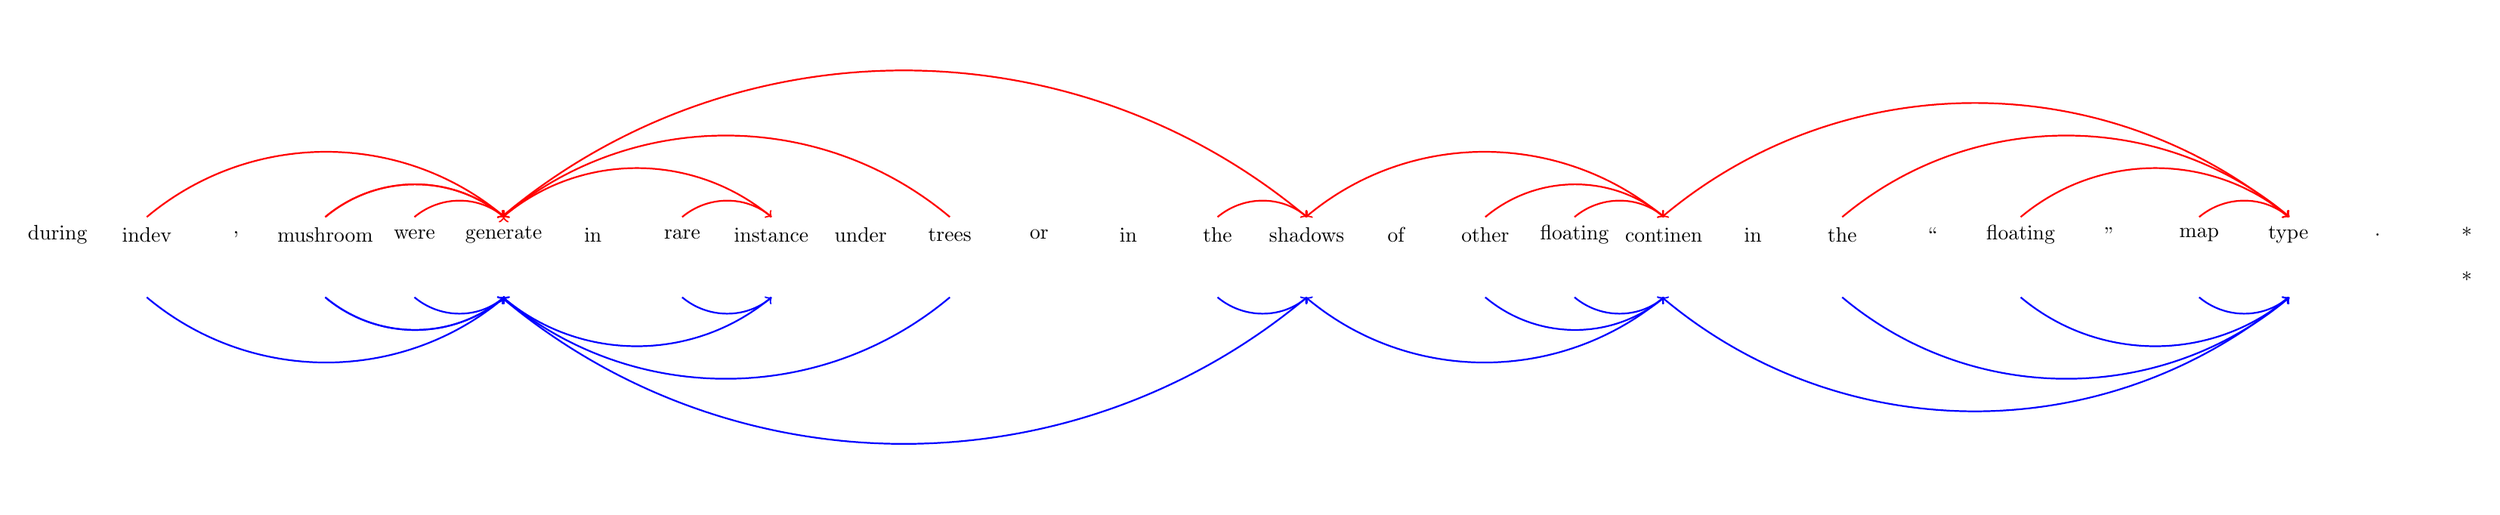
\begin{tikzpicture}[scale=1.5]
\draw(0,0) node {during};
\draw(0,-0.5) node {};
\draw(1,0) node {indev};
\draw(1,-0.5) node {};
\draw(2,0) node {,};
\draw(2,-0.5) node {};
\draw(3,0) node {mushroom};
\draw(3,-0.5) node {};
\draw(4,0) node {were};
\draw(4,-0.5) node {};
\draw(5,0) node {generate};
\draw(5,-0.5) node {};
\draw(6,0) node {in};
\draw(6,-0.5) node {};
\draw(7,0) node {rare};
\draw(7,-0.5) node {};
\draw(8,0) node {instance};
\draw(8,-0.5) node {};
\draw(9,0) node {under};
\draw(9,-0.5) node {};
\draw(10,0) node {trees};
\draw(10,-0.5) node {};
\draw(11,0) node {or};
\draw(11,-0.5) node {};
\draw(12,0) node {in};
\draw(12,-0.5) node {};
\draw(13,0) node {the};
\draw(13,-0.5) node {};
\draw(14,0) node {shadows};
\draw(14,-0.5) node {};
\draw(15,0) node {of};
\draw(15,-0.5) node {};
\draw(16,0) node {other};
\draw(16,-0.5) node {};
\draw(17,0) node {floating};
\draw(17,-0.5) node {};
\draw(18,0) node {continen};
\draw(18,-0.5) node {};
\draw(19,0) node {in};
\draw(19,-0.5) node {};
\draw(20,0) node {the};
\draw(20,-0.5) node {};
\draw(21,0) node {``};
\draw(21,-0.5) node {};
\draw(22,0) node {floating};
\draw(22,-0.5) node {};
\draw(23,0) node {''};
\draw(23,-0.5) node {};
\draw(24,0) node {map};
\draw(24,-0.5) node {};
\draw(25,0) node {type};
\draw(25,-0.5) node {};
\draw(26,0) node {.};
\draw(26,-0.5) node {};
\draw(27,0) node {*};
\draw(27,-0.5) node {*};
\draw[thick,red,->] (1,0.2) arc(130:50:3.12);
\draw[thick,red,->] (3,0.2) arc(130:50:1.56);
\draw[thick,red,->] (3,0.2) arc(130:50:1.56);
\draw[thick,red,->] (4,0.2) arc(130:50:0.78);
\draw[thick,red,->] (5,0.2) arc(50:130:0.0);
\draw[thick,red,->] (7,0.2) arc(130:50:0.78);
\draw[thick,red,->] (8,0.2) arc(50:130:2.34);
\draw[thick,red,->] (10,0.2) arc(50:130:3.9);
\draw[thick,red,->] (13,0.2) arc(130:50:0.78);
\draw[thick,red,->] (14,0.2) arc(50:130:7.02);
\draw[thick,red,->] (16,0.2) arc(130:50:1.56);
\draw[thick,red,->] (17,0.2) arc(130:50:0.78);
\draw[thick,red,->] (18,0.2) arc(50:130:3.12);
\draw[thick,red,->] (20,0.2) arc(130:50:3.9);
\draw[thick,red,->] (22,0.2) arc(130:50:2.34);
\draw[thick,red,->] (24,0.2) arc(130:50:0.78);
\draw[thick,red,->] (25,0.2) arc(50:130:5.46);
\draw[thick,blue,->] (1,-0.7) arc(50:130:-3.12);
\draw[thick,blue,->] (3,-0.7) arc(50:130:-1.56);
\draw[thick,blue,->] (3,-0.7) arc(50:130:-1.56);
\draw[thick,blue,->] (4,-0.7) arc(50:130:-0.78);
\draw[thick,blue,->] (5,-0.7) arc(130:50:-0.0);
\draw[thick,blue,->] (7,-0.7) arc(50:130:-0.78);
\draw[thick,blue,->] (8,-0.7) arc(130:50:-2.34);
\draw[thick,blue,->] (10,-0.7) arc(130:50:-3.9);
\draw[thick,blue,->] (13,-0.7) arc(50:130:-0.78);
\draw[thick,blue,->] (14,-0.7) arc(130:50:-7.02);
\draw[thick,blue,->] (16,-0.7) arc(50:130:-1.56);
\draw[thick,blue,->] (17,-0.7) arc(50:130:-0.78);
\draw[thick,blue,->] (18,-0.7) arc(130:50:-3.12);
\draw[thick,blue,->] (20,-0.7) arc(50:130:-3.9);
\draw[thick,blue,->] (22,-0.7) arc(50:130:-2.34);
\draw[thick,blue,->] (24,-0.7) arc(50:130:-0.78);
\draw[thick,blue,->] (25,-0.7) arc(130:50:-5.46);
\end{tikzpicture}
\end{center}

\end{document}